% =============================================================================
% TOYSOUND-01 Architecture and Engineering Feasibility Study
% LaTeX Source — Compile with: pdflatex -interaction=nonstopmode toysound_arch.tex
% Requires: tikz, pgf, booktabs, longtable, hyperref, geometry, listings, xcolor
% =============================================================================
\documentclass[11pt,a4paper]{article}

% ---------- Packages ----------
\usepackage[margin=25mm]{geometry}
\usepackage[T1]{fontenc}
\usepackage[utf8]{inputenc}
\usepackage{lmodern}
\usepackage{microtype}
\usepackage{amsmath}
\usepackage{amssymb}
\usepackage{xcolor}
\usepackage{graphicx}
\usepackage{booktabs}
\usepackage{longtable}
\usepackage{array}
\usepackage{tabularx}
\usepackage{multirow}
\usepackage{tikz}
\usetikzlibrary{shapes.geometric, arrows.meta, positioning, fit, backgrounds,
                calc, decorations.pathreplacing}
\usepackage{pgfplots}
\pgfplotsset{compat=1.18}
\usepackage{listings}
\usepackage{fancyhdr}
\usepackage{titlesec}
\usepackage{enumitem}
\usepackage{caption}
\usepackage{subcaption}
\usepackage[hidelinks]{hyperref}
\usepackage{tocloft}
\usepackage{float}
\usepackage{mdframed}
\usepackage{pifont}

% ---------- Colours ----------
\definecolor{frozen}{RGB}{0,100,0}
\definecolor{proposed}{RGB}{180,100,0}
\definecolor{unknown}{RGB}{150,0,0}
\definecolor{open}{RGB}{0,0,160}
\definecolor{codegray}{RGB}{245,245,245}
\definecolor{codeblue}{RGB}{0,0,200}
\definecolor{headerblue}{RGB}{30,70,130}
\definecolor{riskred}{RGB}{200,50,50}
\definecolor{riskamb}{RGB}{200,150,0}
\definecolor{riskgrn}{RGB}{50,150,50}

% ---------- Status badges ----------
\newcommand{\frozen}{\textcolor{frozen}{\textbf{[FROZEN]}}}
\newcommand{\proposed}{\textcolor{proposed}{\textbf{[PROPOSED]}}}
\newcommand{\unknown}{\textcolor{unknown}{\textbf{[UNKNOWN]}}}
\newcommand{\openitem}{\textcolor{open}{\textbf{[OPEN]}}}
\newcommand{\confirmed}{\textcolor{frozen}{\textbf{[CONFIRMED]}}}
\newcommand{\blocked}{\textcolor{unknown}{\textbf{[BLOCKED]}}}
\newcommand{\assumption}{\textcolor{proposed}{\textbf{[ASSUMPTION]}}}

% ---------- Code style ----------
\lstset{
  basicstyle=\ttfamily\small,
  backgroundcolor=\color{codegray},
  frame=single,
  framesep=3pt,
  breaklines=true,
  captionpos=b,
  keywordstyle=\color{codeblue}\bfseries,
  commentstyle=\color{gray},
  numbers=left,
  numberstyle=\tiny\color{gray},
  numbersep=5pt,
  tabsize=2
}

% ---------- Header / Footer ----------
\pagestyle{fancy}
\fancyhf{}
\fancyhead[L]{\small\textbf{TOYSOUND-01} --- Architecture \& Feasibility Study}
\fancyhead[R]{\small SCL 1.2~\textmu m C1D PDK}
\fancyfoot[C]{\small\thepage}
\fancyfoot[R]{\small CONFIDENTIAL --- v1.0 --- 2026-11-03}
\renewcommand{\headrulewidth}{0.4pt}

% ---------- Section formatting ----------
\titleformat{\section}{\large\bfseries\color{headerblue}}{{\thesection}}{1em}{}
\titleformat{\subsection}{\normalsize\bfseries}{{\thesubsection}}{1em}{}
\titleformat{\subsubsection}{\normalsize\itshape}{{\thesubsubsection}}{1em}{}

% ---------- TikZ block styles ----------
\tikzstyle{block} = [rectangle, draw, fill=blue!10, text centered,
                     minimum height=1.8em, minimum width=5em, font=\small]
\tikzstyle{analog} = [rectangle, draw, fill=orange!20, text centered,
                      minimum height=1.8em, minimum width=5em, font=\small,
                      dashed]
\tikzstyle{padblock} = [rectangle, draw, fill=green!15, text centered,
                        minimum height=1.8em, minimum width=4em, font=\scriptsize]
\tikzstyle{arrow} = [thick,->,>=stealth]
\tikzstyle{darrow} = [thick,<->,>=stealth]

% =============================================================================
\begin{document}
% =============================================================================

% ---------- Title page ----------
\begin{titlepage}
  \centering
  \vspace*{2cm}
  {\huge\bfseries\color{headerblue} TOYSOUND-01}\\[0.5em]
  {\Large Architecture and Engineering Feasibility Study}\\[0.5em]
  {\large of a Single-Button Four-Tone ASIC}\\[0.3em]
  {\large Using the SCL 1.2~\textmu m C1D PDK}\\[2em]

  \rule{\textwidth}{1pt}\\[1em]

  \begin{tabular}{ll}
    \textbf{Document:}   & TOYSOUND\_01\_ARCHITECTURE\_SPECIFICATION \\
    \textbf{Version:}    & 1.0 \\
    \textbf{Date:}       & 2026-11-03 \\
    \textbf{Process:}    & SCL 1.2~\textmu m CMOS (C1D) \\
    \textbf{PDK source:} & eChipHub / NIELIT \\
    \textbf{Status:}     & \textcolor{proposed}{\textbf{UNDER REVIEW --- Pending owner approval}} \\
    \textbf{Author:}     & Arpit Tiwari \\
    \textbf{Project:}    & COB --- 01\_toysound \\
  \end{tabular}

  \vspace{2em}
  \rule{\textwidth}{1pt}

  \vspace{1em}
  \begin{mdframed}[backgroundcolor=riskamb!10,linecolor=riskamb]
    \centering
    \textbf{STOP NOTICE:} This document is an architecture and feasibility study only.\\
    RTL implementation has \emph{not} been approved at this stage.\\
    Wait for explicit owner approval before writing production RTL.
  \end{mdframed}

  \vfill
  {\small Generated by Antigravity --- HP Victus / Windows 11 / WSL2 (pending) --- MiKTeX 4.23}
\end{titlepage}

% ---------- Table of Contents ----------
\tableofcontents
\newpage

% =============================================================================
\section{Executive Summary}
% =============================================================================

TOYSOUND-01 is a low-cost single-button four-tone ASIC designed for simple electronic toys.
The device uses the SCL 1.2~\textmu m C1D process available through eChipHub/NIELIT.
It generates one of four square-wave audio frequencies on demand, cycling through states
on successive button presses: OFF, Tone~1 (500~Hz), Tone~2 (700~Hz), Tone~3 (900~Hz),
Tone~4 (1200~Hz), and back to OFF.

The architecture has been designed with minimum silicon area, minimum component count, and
low manufacturing complexity as the primary objectives. No external crystal, PLL, or dedicated
reset pin is required in the proposed architecture, subject to validation.

\subsection*{Key findings from PDK inspection}

The SCL C1D PDK has been physically inspected. The following components are confirmed present:
Liberty files (TYP/MAX/MIN), LEF files (core, I/O, tech, corner), GDS libraries (core, I/O),
Verilog cell models, CDL netlists, KLayout DRC and LVS decks, OpenRCX parasitic extraction model,
OpenLane/OpenROAD script templates, and pre-verified pad frames (1--5~mm square).

\subsection*{Critical open issues}

\begin{enumerate}[label=\textbf{\color{unknown}\Alph*.}]
  \item \textbf{Functional specification ambiguity:} The approved specification requires a
    continuous-tone hold-active architecture (each press selects a continuous tone).
    The existing RTL implements a one-shot melody sequencer. These are architecturally
    incompatible. Owner confirmation is required before RTL can proceed.

  \item \textbf{Internal oscillator not yet validated:} The analog PDK zip has not been
    extracted. SPICE device models are unconfirmed. No oscillator circuit has been designed
    or simulated. A clock source is a fundamental silicon requirement.

  \item \textbf{WSL2 not installed:} All Linux EDA tools (iverilog, Yosys, OpenLane, KLayout,
    Ngspice) require WSL2 Ubuntu 22.04. This is the highest-priority setup task.

  \item \textbf{POR circuit not designed:} Standard-cell flip-flops do not have guaranteed
    power-up state. An explicit power-on-reset circuit is required and must be designed at
    transistor level.
\end{enumerate}

% =============================================================================
\section{Product Concept and Design Objectives}
% =============================================================================

\subsection{Product Concept}

TOYSOUND-01 is a bare-die ASIC for chip-on-board (COB) assembly in simple electronic toys.
A single push button advances through five states: silence and four distinct audio tones.
The output drives a piezoelectric buzzer or a small speaker through an appropriate external
driver. No external clock, crystal, or PLL is required.

\subsection{Design Objectives (Priority Order)}

\begin{enumerate}
  \item Minimum silicon area
  \item Minimum component count on PCB
  \item Low power consumption (battery-operated toy)
  \item Simple PCB integration
  \item Low manufacturing complexity
  \item Reliable power-up behaviour
  \item Easy functional verification
  \item Manufacturable physical layout
  \item Clear technical explanation for semiconductor interviews
\end{enumerate}

% =============================================================================
\section{Frozen Functional Requirements}
% =============================================================================

\begin{table}[H]
  \centering
  \caption{Frozen functional decisions}
  \begin{tabularx}{\textwidth}{lX}
    \toprule
    \textbf{Parameter} & \textbf{Decision} \\
    \midrule
    User input          & One push button \frozen \\
    Button operation    & Cycle through five states \frozen \\
    Operating states    & OFF, Tone~1, Tone~2, Tone~3, Tone~4 \frozen \\
    Output waveform     & Square wave \frozen \\
    Number of tones     & Four \frozen \\
    Clock source        & Internal oscillator \proposed \\
    Crystal             & Not required \proposed \\
    PLL                 & Not required \frozen \\
    External clock pin  & Not required \proposed \\
    Output              & One sound output \frozen \\
    Process             & SCL 1.2~\textmu m C1D \frozen \\
    \bottomrule
  \end{tabularx}
\end{table}

\subsection{Button Operating Sequence}

\begin{center}
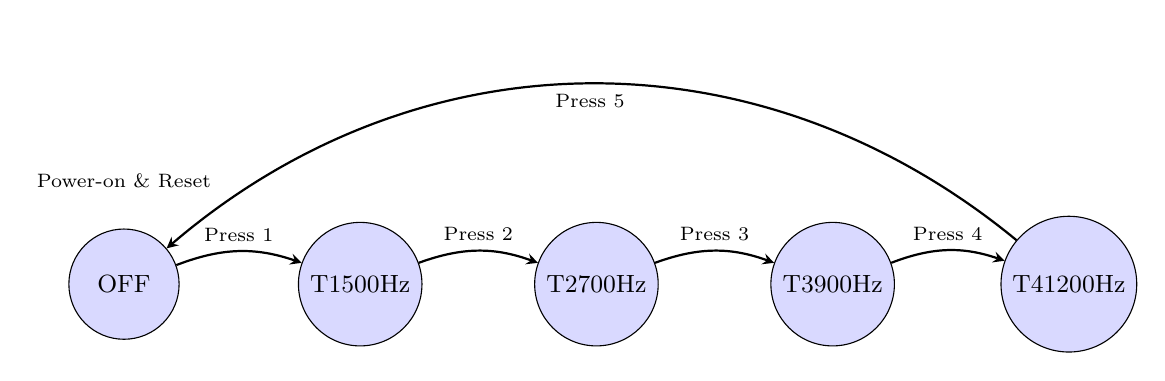
\begin{tikzpicture}[node distance=1.8cm, auto]
  \tikzstyle{state}=[circle, draw, fill=blue!15, minimum size=1.4cm,
                     font=\small, text centered]
  \tikzstyle{arc}=[thick,->,>=stealth,bend left=20]
  \tikzstyle{labl}=[font=\scriptsize,above]

  \node[state] (OFF)  at (0,0)    {OFF};
  \node[state] (T1)   at (3,0)    {T1\\500Hz};
  \node[state] (T2)   at (6,0)    {T2\\700Hz};
  \node[state] (T3)   at (9,0)    {T3\\900Hz};
  \node[state] (T4)   at (12,0)   {T4\\1200Hz};

  \draw[arc] (OFF) to node[labl]{Press 1} (T1);
  \draw[arc] (T1)  to node[labl]{Press 2} (T2);
  \draw[arc] (T2)  to node[labl]{Press 3} (T3);
  \draw[arc] (T3)  to node[labl]{Press 4} (T4);
  \draw[->,thick,>=stealth,bend right=40] (T4) to node[below,font=\scriptsize]{Press 5} (OFF);
  \node[above=0.4cm of OFF,font=\scriptsize] {Power-on \& Reset};
\end{tikzpicture}
\end{center}

One valid press generates exactly one state transition. A held button does not advance the
selection. Mechanical bounce is suppressed by an on-chip debounce counter.

% =============================================================================
\section{System Block Diagram}
% =============================================================================

\begin{figure}[H]
  \centering
  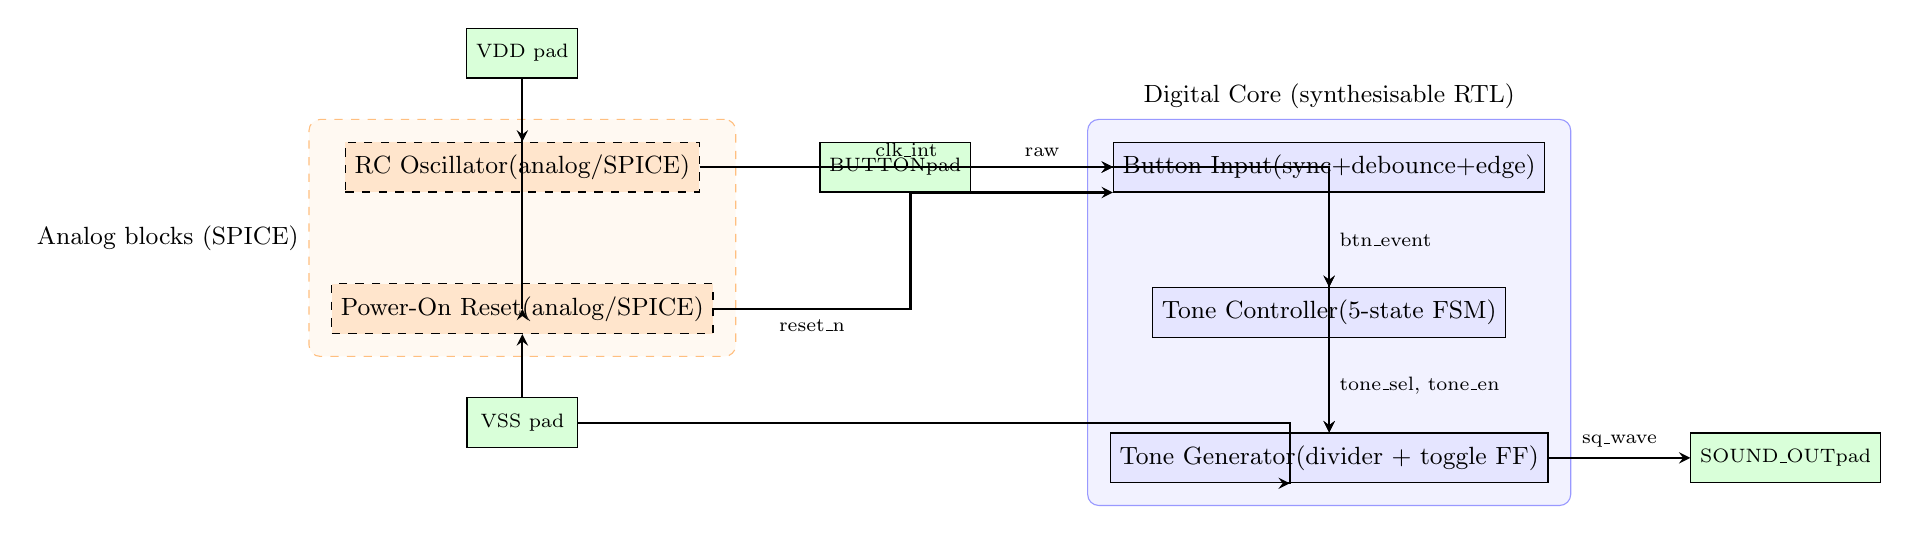
\begin{tikzpicture}[node distance=1.2cm and 2cm]

    % --- Analog blocks ---
    \node[analog, minimum width=3cm] (osc)  at (0,0)    {RC Oscillator\\(analog/SPICE)};
    \node[analog, minimum width=3cm] (por)  at (0,-1.8) {Power-On Reset\\(analog/SPICE)};

    % --- Digital blocks ---
    \node[block, right=2.5cm of osc, minimum width=3.5cm] (btn) at (5,0)
          {Button Input\\(sync+debounce+edge)};
    \node[block, below=1.2cm of btn, minimum width=3.5cm] (ctrl)
          {Tone Controller\\(5-state FSM)};
    \node[block, below=1.2cm of ctrl, minimum width=3.5cm] (tgen)
          {Tone Generator\\(divider + toggle FF)};

    % --- Pads ---
    \node[padblock, left=1.8cm of btn]  (btnpad)  {BUTTON\\pad};
    \node[padblock, right=1.8cm of tgen](outpad)  {SOUND\_OUT\\pad};
    \node[padblock, above=0.8cm of osc] (vddpad)  {VDD pad};
    \node[padblock, below=0.8cm of por] (vsspad)  {VSS pad};

    % --- Arrows ---
    \draw[arrow] (osc)    -- node[above,font=\scriptsize]{clk\_int} (btn);
    \draw[arrow] (osc)    -| node[near start,right,font=\scriptsize]{} (ctrl);
    \draw[arrow] (osc)    -| node[near start,right,font=\scriptsize]{} (tgen);
    \draw[arrow] (por)    -- node[below,font=\scriptsize]{reset\_n}
                    ([xshift=2.5cm]por.east) |- (btn.south west);
    \draw[arrow] (btnpad) -- node[above,font=\scriptsize]{raw} (btn);
    \draw[arrow] (btn)    -- node[right,font=\scriptsize]{btn\_event} (ctrl);
    \draw[arrow] (ctrl)   -- node[right,font=\scriptsize]{tone\_sel, tone\_en} (tgen);
    \draw[arrow] (tgen)   -- node[above,font=\scriptsize]{sq\_wave} (outpad);
    \draw[arrow] (vddpad) -- (osc);
    \draw[arrow] (vddpad) |- (por);
    \draw[arrow] (vsspad) -- (por);
    \draw[arrow] (vsspad) -| ([xshift=-0.5cm]tgen.south) -- (tgen);

    % --- Digital core bounding box ---
    \begin{scope}[on background layer]
      \node[draw=blue!40, fill=blue!5, fit=(btn)(ctrl)(tgen),
            inner sep=8pt, rounded corners, label=above:{\small Digital Core (synthesisable RTL)}] {};
    \end{scope}

    % --- Analog bounding box ---
    \begin{scope}[on background layer]
      \node[draw=orange!50, fill=orange!5, fit=(osc)(por),
            inner sep=8pt, rounded corners, dashed,
            label=left:{\small Analog blocks (SPICE)}] {};
    \end{scope}

  \end{tikzpicture}
  \caption{TOYSOUND-01 system block diagram (proposed architecture)}
  \label{fig:blockdiag}
\end{figure}

% =============================================================================
\section{Clock Architecture}
% =============================================================================

\subsection{Requirement}

The design must not require an external crystal or PLL. An internal oscillator must generate a
clock of approximately 1~MHz.

\subsection{Oscillator Topology Comparison}

\begin{table}[H]
  \centering
  \caption{Oscillator topology comparison for SCL 1.2~\textmu m CMOS}
  \scriptsize
  \begin{tabularx}{\textwidth}{p{3cm}XXXXX}
    \toprule
    \textbf{Criterion}        & \textbf{CMOS Ring Osc} & \textbf{Current-Starved Ring} &
                                \textbf{RC Relaxation} & \textbf{Schmitt RC} \\
    \midrule
    Transistor count          & 6--12 & 8--20 & 12--24 & 6--12 \\
    Passive components        & None  & None  & R + C  & R + C \\
    Silicon area              & Very small & Small & Medium & Small \\
    PVT frequency variation   & $\pm$40--50\% & $\pm$20--30\% & $\pm$10--20\% & $\pm$15--25\% \\
    Supply sensitivity        & High  & Medium & Lower  & Medium \\
    Temperature sensitivity   & High  & Medium & Lower  & Medium \\
    Startup reliability       & Good  & Good  & Conditional & Good \\
    Layout complexity         & Simple & Simple & Medium & Simple \\
    Passives in SCL PDK       & N/A   & N/A   & \unknown & \unknown \\
    Suitability for toy app   & Marginal (freq. error) & Better & Preferred & Good fallback \\
    \bottomrule
  \end{tabularx}
\end{table}

\subsection{Recommendation}

An \textbf{RC relaxation oscillator or Schmitt-trigger RC oscillator} is preferred over a
plain ring oscillator because of superior PVT stability. However, this requires on-chip resistor
and capacitor models.

\begin{mdframed}[backgroundcolor=unknown!10,linecolor=unknown]
  \textbf{BLOCKED:} The SCL 1.2~\textmu m analog PDK archive (\texttt{Open\_Source\_SCL\_1.2micron\_PDK.zip})
  has not been extracted. NMOS, PMOS, resistor, and capacitor SPICE models are unconfirmed.
  No oscillator topology can be finally selected or designed until this step is completed.
\end{mdframed}

\subsection{Critical Distinction: Simulation Clock vs Physical Oscillator}

\begin{mdframed}[backgroundcolor=riskred!10,linecolor=riskred]
  \textbf{Engineering rule:} A Verilog construct such as \texttt{always \#500 clk = \~{}clk;}
  is a simulation model only. It has zero physical meaning. It cannot be synthesised and placed
  in a real design. The physical oscillator must be designed at transistor level in SPICE and
  implemented as custom analog layout. An RTL model with idealised delays cannot be called an
  oscillator. Using such a model in synthesis would produce a design without a clock source.
\end{mdframed}

\subsection{Effect of Oscillator Frequency Error on Tone Accuracy}

If the actual oscillator frequency is $f_{clk}' = f_{clk}(1+\varepsilon)$, where $\varepsilon$
is the fractional frequency error due to PVT variation, then all output tones scale equally:
\begin{equation}
  f_{out}' = \frac{f_{clk}'}{2N} = f_{out}(1+\varepsilon)
\end{equation}
The ratio between tones is preserved. For a toy audio application, a $\pm20\%$ error is audibly
significant but not necessarily a product-failure criterion. The product requirement for tone
accuracy must be defined.

% =============================================================================
\section{Frequency Divider Calculations}
% =============================================================================

\begin{equation}
  f_{out} = \frac{f_{clk}}{2N}
  \quad \Rightarrow \quad
  N = \frac{f_{clk}}{2 \cdot f_{out}}
\end{equation}

At $f_{clk} = 1$~MHz nominal:

\begin{table}[H]
  \centering
  \caption{Tone frequency calculations at 1~MHz clock}
  \begin{tabular}{lrrrrr}
    \toprule
    \textbf{Tone} & \textbf{Target (Hz)} & \textbf{N (exact)} & \textbf{N (integer)} &
    \textbf{Actual (Hz)} & \textbf{Error (\%)} \\
    \midrule
    Tone 1 & 500   & 1000.000 & 1000 & 500.00   & $0.000\%$ \\
    Tone 2 & 700   & 714.286  & 714  & 700.280  & $+0.040\%$ \\
    Tone 3 & 900   & 555.556  & 556  & 899.281  & $-0.080\%$ \\
    Tone 4 & 1200  & 416.667  & 417  & 1199.041 & $-0.080\%$ \\
    \bottomrule
  \end{tabular}
\end{table}

All quantisation errors are below $0.1\%$ --- negligible for audio in a toy application.
The dominant frequency error source is oscillator PVT variation, not quantisation.

\textbf{Counter bit width:} Maximum $N = 1000$; required width $= \lceil \log_2(1000) \rceil = 10$~bits.

\textbf{Duty cycle:} Exactly 50\% by design. The output toggles at each terminal count, producing
equal high and low half-periods of $N$ clock cycles each.

% =============================================================================
\section{Power-On Reset Architecture}
% =============================================================================

\subsection{Requirement}

The digital controller must initialise reliably to the OFF state after power-up.
Standard-cell flip-flops in CMOS processes \textbf{do not} have a guaranteed power-up state.
An explicit transistor-level POR circuit is required.

\subsection{Proposed POR Circuit Concept}

\begin{figure}[H]
  \centering
  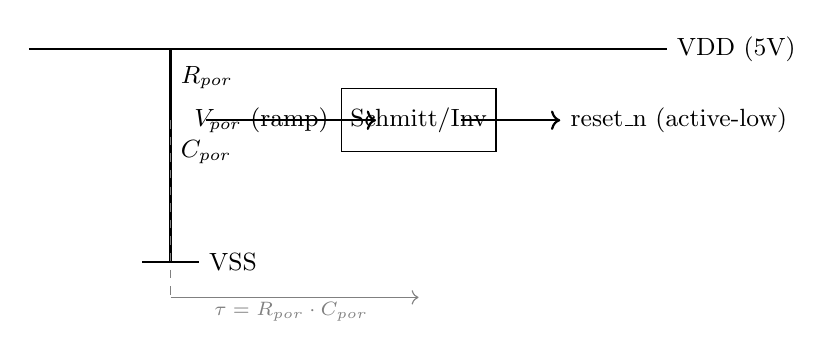
\begin{tikzpicture}[scale=0.9]
    % VDD rail
    \draw[thick] (-1,3) -- (8,3) node[right]{\small VDD (5V)};
    % Resistor
    \draw[thick] (1,3) -- (1,2.2)
          node[midway,right]{\small $R_{por}$};
    \draw[thick] (1,2.2) -- (1,1.8);
    % Capacitor
    \draw[thick] (1,1.8) -- (1,1.3)
          node[midway,right]{\small $C_{por}$};
    \draw[thick] (1,1.3) -- (1,0.8);
    % Ground
    \draw[thick] (1,0.8) -- (1,0);
    \draw[thick] (0.6,0) -- (1.4,0) node[right]{\small VSS};
    % Node label
    \node[right] at (1.2,2.0) {\small $V_{por}$ (ramp)};
    % Inverter chain (POR output)
    \node[draw,minimum width=1.2cm, minimum height=0.8cm] at (4.5,2.0) {\small Schmitt/Inv};
    \draw[thick,->] (1.5,2.0) -- (3.9,2.0);
    \draw[thick,->] (5.1,2.0) -- (6.5,2.0) node[right]{\small reset\_n (active-low)};
    % Timing annotation
    \draw[dashed,gray] (1,2.0) -- (1,-0.5);
    \draw[->,gray] (1,-0.5) -- (4.5,-0.5);
    \node[gray,font=\scriptsize] at (2.7,-0.7) {$\tau = R_{por} \cdot C_{por}$};
  \end{tikzpicture}
  \caption{Conceptual power-on reset circuit (transistor-level implementation required)}
\end{figure}

The RC time constant determines the reset pulse width. For a 100~µs target reset:
\[
  \tau = R_{por} \cdot C_{por} \geq 100~\text{µs}
\]
Example: $R = 100~\text{k}\Omega$, $C = 1~\text{pF}$ gives $\tau = 0.1$~µs (too short).
Practical values depend on available component models. The actual component values must be
derived from SPICE simulation after the analog PDK is extracted.

\subsection{Reset Polarity and Behaviour}

\begin{itemize}
  \item \textbf{Polarity:} Active-low (\texttt{reset\_n}). This matches the existing RTL.
  \item \textbf{Initial state after reset:} All FSM registers cleared to zero (OFF state).
  \item \textbf{Output during reset:} \texttt{sound\_out = 0} (silence).
  \item \textbf{Button during reset:} Any button press during the reset period is discarded.
        The debounce counter is reset to its initial state.
\end{itemize}

% =============================================================================
\section{Button Input Architecture}
% =============================================================================

\subsection{Circuit Overview}

\begin{figure}[H]
  \centering
  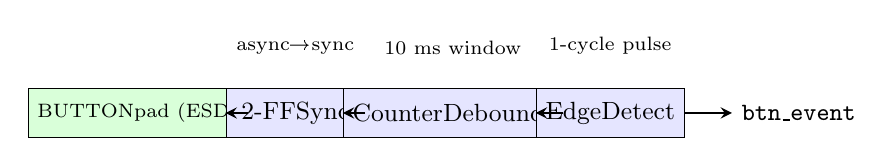
\begin{tikzpicture}[node distance=2cm and 0.8cm, auto]
    \node[padblock] (pad)   {BUTTON\\pad (ESD)};
    \node[block, right of=pad] (sync)  {2-FF\\Sync};
    \node[block, right of=sync] (deb)  {Counter\\Debounce};
    \node[block, right of=deb] (edge) {Edge\\Detect};
    \node[right=0.6cm of edge, font=\small] (out) {\texttt{btn\_event}};

    \draw[arrow] (pad)  -- (sync);
    \draw[arrow] (sync) -- (deb);
    \draw[arrow] (deb)  -- (edge);
    \draw[arrow] (edge) -- (out);

    \node[above=0.3cm of sync, font=\scriptsize] {async→sync};
    \node[above=0.3cm of deb, font=\scriptsize]  {10~ms window};
    \node[above=0.3cm of edge, font=\scriptsize] {1-cycle pulse};
  \end{tikzpicture}
  \caption{Button input processing chain}
\end{figure}

\subsection{Two-FF Synchroniser}

The raw button signal is asynchronous. Directly sampling it can cause metastability.
Two cascaded D flip-flops clocked by \texttt{clk\_int} resolve metastability within two clock
cycles. At 1~MHz, metastability resolution time is approximately $2/f_{clk} = 2$~µs, well within
any human reaction time.

\subsection{Debounce Counter}

\textbf{Proposed debounce interval:} 10~ms = 10,000 clock cycles at 1~MHz. \proposed

\textbf{Counter width:} $\lceil \log_2(10000) \rceil = 14$~bits.

\textbf{Behaviour:}
\begin{itemize}
  \item Counter increments while button held low (pressed).
  \item Counter resets to zero if button bounces high before reaching terminal count.
  \item At terminal count: one \texttt{btn\_event} pulse is generated; counter disarmed.
  \item Counter re-arms only after button is released (returns to logic-1).
\end{itemize}

This ensures: (1)~no double-fire on bounce; (2)~no repeated fire on long press.

\begin{mdframed}[backgroundcolor=riskamb!10,linecolor=riskamb]
  \textbf{Warning:} The current RTL uses \texttt{DEBOUNCE\_CYCLES = 1000} (1~ms). Standard
  mechanical push-button contacts typically produce bounce lasting 5--20~ms. The RTL parameter
  must be updated to 10,000 cycles. Owner confirmation required.
\end{mdframed}

% =============================================================================
\section{Tone Generator Architecture}
% =============================================================================

\subsection{Design Principle}

One shared frequency divider services all four tones. When the tone controller selects a tone,
it loads the corresponding divider value $N$ into the counter. The counter decrements each clock
cycle. At terminal count, the counter reloads and the output toggles. No independent tone
generators are used.

\begin{figure}[H]
  \centering
  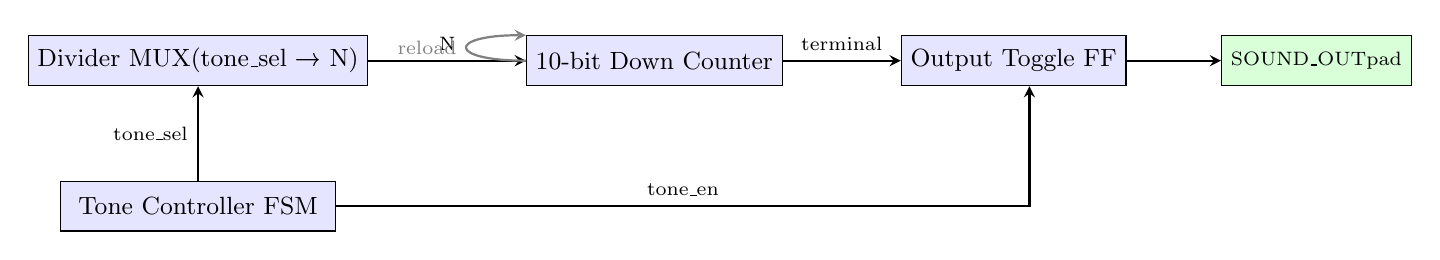
\begin{tikzpicture}[node distance=1.5cm and 2cm]
    \node[block, minimum width=3.5cm] (mux)  {Divider MUX\\(tone\_sel → N)};
    \node[block, right=2cm of mux, minimum width=3cm] (cnt)
          {10-bit Down Counter};
    \node[block, right=1.5cm of cnt, minimum width=2.5cm] (tog)
          {Output Toggle FF};
    \node[padblock, right=1.2cm of tog] (out) {SOUND\_OUT\\pad};
    \node[block, below=1.2cm of mux, minimum width=3.5cm] (ctrl)
          {Tone Controller FSM};

    \draw[arrow] (mux)  -- node[above,font=\scriptsize]{N} (cnt);
    \draw[arrow] (cnt)  -- node[above,font=\scriptsize]{terminal} (tog);
    \draw[arrow] (tog)  -- (out);
    \draw[arrow] (ctrl) -- node[left,font=\scriptsize]{tone\_sel} (mux);
    \draw[arrow] (ctrl.east) -| node[near start,above,font=\scriptsize]{tone\_en}
                    ([xshift=0.2cm]tog.south);
    \draw[->,thick,>=stealth,gray] (cnt.west) .. controls +(west:1) and +(west:1)
        .. node[left,font=\scriptsize]{reload} (cnt.north west);
  \end{tikzpicture}
  \caption{Shared frequency divider architecture (continuous-tone mode)}
\end{figure}

\subsection{Output Enable}

When the FSM is in the OFF state, \texttt{tone\_en = 0} and the output is held at logic-0
(silence). The divider counter is also reset to zero.

\subsection{Continuous Tone vs One-Shot Melody (ADL-017)}

\begin{mdframed}[backgroundcolor=unknown!10,linecolor=unknown]
  \textbf{Critical open decision:} The approved specification requires a \emph{continuous-tone}
  architecture. The existing RTL implements a \emph{one-shot melody sequencer}. These require
  fundamentally different FSM designs. Owner approval is required before RTL can proceed.
\end{mdframed}

% =============================================================================
\section{Output and PCB Interface}
% =============================================================================

\subsection{Output Driver Options}

\begin{table}[H]
  \centering
  \caption{Sound transducer comparison}
  \begin{tabular}{p{3.5cm}p{3.5cm}p{3.5cm}p{2.5cm}}
    \toprule
    \textbf{Parameter} & \textbf{Piezoelectric buzzer} &
    \textbf{Magnetic buzzer/speaker} & \textbf{Decision} \\
    \midrule
    Typical impedance & $>1$~k$\Omega$ (capacitive) & 8--32~$\Omega$ (resistive+inductive) &
    \multirow{4}{*}{\openitem} \\
    Typical peak current (5~V) & $<1$~mA & 150--600~mA & \\
    Direct pad drive possible? & Possibly & No --- driver required & \\
    PCB components needed & None (possibly) & NPN transistor + resistor & \\
    \bottomrule
  \end{tabular}
\end{table}

\subsection{PCB Interface Schematic}

\begin{figure}[H]
  \centering
  \begin{tikzpicture}[scale=0.85]
    % ASIC box
    \draw[thick, fill=blue!8] (3,1) rectangle (7,6);
    \node[font=\small\bfseries] at (5,5.6) {TOYSOUND-01};
    \node[font=\scriptsize] at (5,5.2) {ASIC (COB)};

    % Pads inside
    \node[font=\scriptsize] at (3.6,4.5) {VDD};
    \node[font=\scriptsize] at (3.6,3.5) {VSS};
    \node[font=\scriptsize] at (3.6,2.8) {BTN};
    \node[font=\scriptsize] at (6.4,2.5) {OUT};

    % VDD rail
    \draw[thick] (0,6.5) -- (11,6.5) node[right]{\small VDD (5V)};
    % VSS rail
    \draw[thick] (0,0) -- (11,0) node[right]{\small VSS (GND)};
    % Decoupling cap
    \draw[thick] (1.5,6.5) -- (1.5,5.8) node[midway,right]{\scriptsize 100nF};
    \draw[thick] (1.5,5.8) -- (1.5,5.3);
    \draw[thick] (1.5,5.3) -- (1.5,0);
    % VDD to pad
    \draw[thick,->] (3,6.5) -- (3,4.5) -- (3.5,4.5);
    % VSS to pad
    \draw[thick,->] (3,0) -- (3,3.5) -- (3.5,3.5);
    % Pull-up resistor for button
    \draw[thick] (1,6.5) -- (1,5.0) node[midway,left]{\scriptsize 10k$\Omega$};
    \draw[thick] (1,5.0) -- (1,4.2);
    \node[draw,circle,inner sep=2pt,fill=white] (sw1) at (1,3.8) {};
    \node[font=\scriptsize,left] at (0.7,3.8) {SW1};
    \draw[thick] (1,3.5) -- (1,0);
    % Button to pad
    \draw[thick,->] (1,4.5) -- (3.5,2.8);
    % Output line
    \draw[thick,->] (6.5,2.5) -- (8,2.5);
    % NPN transistor (Option B)
    \node[font=\scriptsize] at (9,2.5) {[1k$\Omega$]};
    \draw[thick] (9.5,2.5) -- (10,2.5) node[right]{\scriptsize Base};
    \draw[thick] (10.3,3.5) -- (10.3,1.5);
    \node[font=\scriptsize,right] at (10.4,3.2) {Collector};
    \node[font=\scriptsize,right] at (10.4,1.8) {Emitter};
    \draw[thick,->] (10.3,3.5) -- (10.3,6.5);
    \node[font=\scriptsize,right] at (10.4,5.0) {[Buzzer]};
    \draw[thick,->] (10.3,1.5) -- (10.3,0);
    \node[font=\scriptsize,above=1cm of sw1,xshift=-0.5cm] {\scriptsize (Mandatory)};
    \node[font=\scriptsize,right=0.5cm of out,yshift=-0.8cm] {\scriptsize (Mandatory for};
    \node[font=\scriptsize,right=0.5cm of out,yshift=-1.2cm] {\scriptsize  magnetic buzzer)};
  \end{tikzpicture}
  \caption{Conceptual PCB interface diagram (Option B: magnetic buzzer with NPN driver)}
\end{figure}

% =============================================================================
\section{Pin Count and Physical Interface}
% =============================================================================

\begin{table}[H]
  \centering
  \caption{Logical signal definition}
  \begin{tabular}{llll}
    \toprule
    \textbf{Signal} & \textbf{Direction} & \textbf{Active state} & \textbf{Purpose} \\
    \midrule
    VDD        & Power   & ---         & Positive supply (5~V nominal) \\
    VSS        & Ground  & ---         & Ground reference \\
    BUTTON     & Input   & Active-low  & User push button \\
    SOUND\_OUT & Output  & Logic-high  & Square-wave audio output \\
    \bottomrule
  \end{tabular}
\end{table}

\begin{table}[H]
  \centering
  \caption{Physical pad count (proposed)}
  \begin{tabular}{llll}
    \toprule
    \textbf{Pad function} & \textbf{PDK pad type} & \textbf{Count} & \textbf{Status} \\
    \midrule
    VDD power pad   & I/O power pad (io\_c1d.lef)   & 1 (min) & \proposed \\
    VSS ground pad  & I/O ground pad (io\_c1d.lef)  & 1 (min) & \proposed \\
    BUTTON input    & Bidirectional/input pad (ESD) & 1        & \proposed \\
    SOUND\_OUT output & Output pad (ESD)             & 1        & \proposed \\
    Corner cells    & corner\_c1d.lef               & 4        & \confirmed \\
    TEST/CLK pad    & Optional input pad            & 0 or 1  & \openitem \\
    \midrule
    \textbf{Total (min)} & & \textbf{8} & \\
    \bottomrule
  \end{tabular}
\end{table}

Available die frame sizes: 1$\times$1, 2$\times$2, 3$\times$3, 4$\times$4, 5$\times$5~mm.
Pre-verified DRC/LVS-clean GDS and CDL provided for all five sizes in the PDK.

% =============================================================================
\section{RTL Module Hierarchy}
% =============================================================================

\begin{figure}[H]
  \centering
  \small
  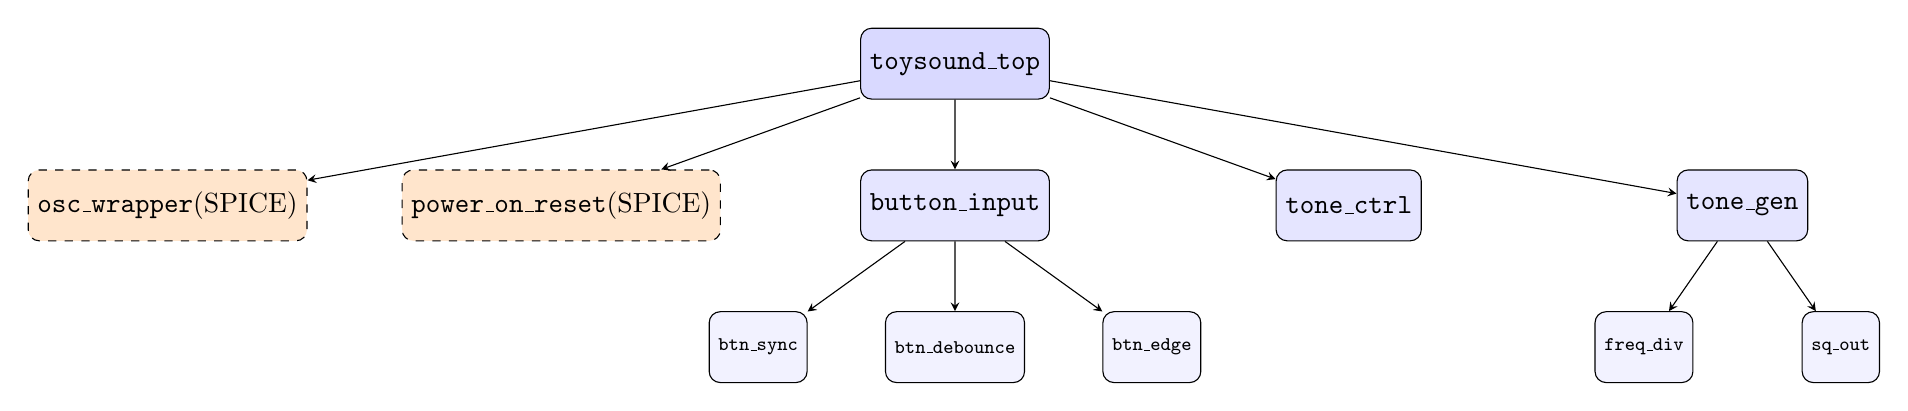
\begin{tikzpicture}[
    every node/.style={draw, rectangle, rounded corners, minimum height=0.9cm},
    level 1/.style={sibling distance=5cm, level distance=1.8cm},
    level 2/.style={sibling distance=2.5cm, level distance=1.8cm},
    edge from parent/.style={draw,->,>=stealth}
  ]
    \node[fill=blue!15] {\texttt{toysound\_top}}
      child { node[fill=orange!20, dashed] {\texttt{osc\_wrapper}\\(SPICE)} }
      child { node[fill=orange!20, dashed] {\texttt{power\_on\_reset}\\(SPICE)} }
      child { node[fill=blue!10] {\texttt{button\_input}}
        child { node[fill=blue!5,font=\scriptsize] {\texttt{btn\_sync}} }
        child { node[fill=blue!5,font=\scriptsize] {\texttt{btn\_debounce}} }
        child { node[fill=blue!5,font=\scriptsize] {\texttt{btn\_edge}} }
      }
      child { node[fill=blue!10] {\texttt{tone\_ctrl}} }
      child { node[fill=blue!10] {\texttt{tone\_gen}}
        child { node[fill=blue!5,font=\scriptsize] {\texttt{freq\_div}} }
        child { node[fill=blue!5,font=\scriptsize] {\texttt{sq\_out}} }
      };
  \end{tikzpicture}
  \caption{RTL module hierarchy (continuous-tone architecture)}
\end{figure}

\begin{table}[H]
  \centering
  \caption{Module implementation classification}
  \scriptsize
  \begin{tabular}{llll}
    \toprule
    \textbf{Module} & \textbf{Type} & \textbf{Tool} & \textbf{Notes} \\
    \midrule
    toysound\_top   & RTL (synthesisable) & Yosys+OpenROAD & Top integration \\
    osc\_wrapper    & Custom/SPICE stub   & Ngspice + layout & Clock source \\
    power\_on\_reset & Custom/SPICE       & Ngspice + layout & POR circuit \\
    button\_sync    & RTL                 & Yosys & 2 FF cascade \\
    button\_debounce & RTL               & Yosys & 14-bit counter \\
    button\_edge    & RTL                 & Yosys & 1 FF + AND \\
    tone\_ctrl      & RTL                 & Yosys & 3-bit FSM \\
    freq\_div       & RTL                 & Yosys & 10-bit counter \\
    sq\_out         & RTL                 & Yosys & Toggle FF + gate \\
    \bottomrule
  \end{tabular}
\end{table}

% =============================================================================
\section{Preliminary Area and Power Estimation Methodology}
% =============================================================================

\begin{mdframed}[backgroundcolor=gray!10]
  \textbf{Note:} Actual area and power values cannot be calculated without completing synthesis
  and place-and-route. The equations below define the estimation methodology and data
  dependencies. No numerical results are fabricated.
\end{mdframed}

\subsection{Area Estimation}

\begin{equation}
  A_{core} = A_{cells} \times (1 + r_{routing})
\end{equation}
where $A_{cells}$ is the sum of standard-cell areas from the Liberty file, and $r_{routing}$ is
the routing area overhead (typically 0.3--0.7 for small designs).

\begin{equation}
  A_{die} = A_{core} + A_{padring}
\end{equation}

The pad ring overhead is fixed by the selected frame size. For a 1$\times$1~mm frame:
$A_{padring}$ is determined by the number and type of I/O pads multiplied by their individual
LEF dimensions.

\textbf{Required data:} Yosys \texttt{stat} report (cell count and area); LEF file (pad dimensions).

\subsection{Power Estimation}

Dynamic power (digital core):
\begin{equation}
  P_{dyn} = \alpha \cdot C_{L} \cdot V_{DD}^2 \cdot f_{clk}
\end{equation}
where $\alpha$ is the activity factor ($\approx 0.1$--$0.2$ for this type of logic),
$C_L$ is the switched capacitance (from Liberty/LEF), $V_{DD} = 5$~V, $f_{clk} = 1$~MHz.

Leakage power: $P_{leak} = N_{cells} \times P_{leak,cell}$ (from Liberty).

Oscillator power: From SPICE transient current measurement (not yet available).

Output load power: $P_{load} = \frac{1}{2} C_{load} V_{DD}^2 f_{out}$ for capacitive load.

% =============================================================================
\section{Testability and DFT}
% =============================================================================

\subsection{Recommendation}

This is a small design (estimated $<500$ gates). A full scan-chain architecture would:
\begin{itemize}
  \item Require an additional test-enable (TE) pin.
  \item Add routing overhead ($10$--$15$\% typical).
  \item Add scan insertion complexity in the EDA flow.
  \item Increase design time disproportionate to the design size.
\end{itemize}

\textbf{Minimum testability proposal:}
\begin{enumerate}
  \item Functional test via BUTTON and SOUND\_OUT pads only.
  \item Optional dedicated CLK\_TEST pad: allows an external clock to be applied during
        wafer probing, bypassing the oscillator.
  \item SOUND\_OUT frequency measured during test to verify all four tone states.
  \item Test sequence: apply 5 button presses; measure SOUND\_OUT frequency at each state.
\end{enumerate}

A single external test clock pin would increase pad count from 8 to 9 but enable significantly
faster and more reliable manufacturing test.

% =============================================================================
\section{PDK Inventory}
% =============================================================================

\begin{table}[H]
  \centering
  \caption{SCL C1D PDK inventory (physically inspected 2026-11-03)}
  \small
  \begin{tabularx}{\textwidth}{llX}
    \toprule
    \textbf{File/Component} & \textbf{Status} & \textbf{Notes} \\
    \midrule
    \texttt{c1d\_core\_typ.lib} & \confirmed & Liberty TYP corner; 5V, 27°C \\
    \texttt{c1d\_core\_max.lib} & \confirmed & Liberty MAX/slow corner \\
    \texttt{c1d\_core\_min.lib} & \confirmed & Liberty MIN/fast corner \\
    \texttt{scl1u\_pads\_*.lib} (3 corners) & \confirmed & I/O pad Liberty files \\
    \texttt{core\_c1d.lef} & \confirmed & Standard cell LEF abstracts \\
    \texttt{tech\_c1d.lef} & \confirmed & Technology LEF \\
    \texttt{io\_c1d.lef} & \confirmed & I/O pad LEF \\
    \texttt{corner\_c1d.lef} & \confirmed & Corner cell LEF \\
    \texttt{core\_c1d.gds} & \confirmed & Standard cell GDS \\
    \texttt{io\_c1d.gds} & \confirmed & I/O pad GDS \\
    \texttt{c1d.v} & \confirmed & Verilog behavioural models \\
    \texttt{core\_iolib\_c1d.cdl} & \confirmed & LVS CDL reference \\
    \texttt{drc.lydrc} & \confirmed & KLayout DRC deck \\
    \texttt{lvs.lylvs} & \confirmed & KLayout LVS deck \\
    \texttt{scl\_c1d.rcx.lib} & \confirmed & OpenRCX parasitic extraction \\
    \texttt{scl\_c1d.map} & \confirmed & DEF$\to$GDS layer map \\
    \texttt{*\_c1d.tcl} scripts (7 stages) & \confirmed & OpenLane/OpenROAD templates \\
    \texttt{verilog2spice.py} & \confirmed & LVS CDL generation utility \\
    Pad frame GDS (1--5~mm) & \confirmed & 5 pre-verified frame sizes \\
    Analog SPICE models (NMOS/PMOS/R/C) & \unknown & Inside unextracted .zip \\
    Device operating ranges & \unknown & In unread reference PDF \\
    ESD HBM specification & \unknown & In unread Standard\_Pad\_Frame PDF \\
    \bottomrule
  \end{tabularx}
\end{table}

% =============================================================================
\section{Toolchain Compatibility Matrix}
% =============================================================================

\begin{table}[H]
  \centering
  \caption{EDA toolchain compatibility (SCL C1D PDK)}
  \scriptsize
  \begin{tabularx}{\textwidth}{p{3cm}p{2.8cm}p{2.5cm}Xp{2cm}}
    \toprule
    \textbf{Stage} & \textbf{Required input} & \textbf{Tool} & \textbf{PDK support} & \textbf{Status} \\
    \midrule
    RTL simulation & \texttt{c1d.v} & iverilog & \confirmed & \blocked (WSL2) \\
    Waveform & VCD & GTKWave & \confirmed & \blocked (WSL2) \\
    Synthesis & Liberty & Yosys 0.9 & \confirmed & \blocked (WSL2) \\
    Floorplan & LEF+Liberty & OpenROAD & \confirmed & \blocked (WSL2) \\
    Placement & LEF+DEF & OpenROAD & \confirmed & \blocked (WSL2) \\
    CTS & Liberty+DEF & OpenROAD & \confirmed & \blocked (WSL2) \\
    Routing & LEF+DEF & OpenROAD & \confirmed & \blocked (WSL2) \\
    DRC & GDS & KLayout 0.30.7 & \confirmed & \blocked (WSL2) \\
    LVS & GDS+CDL & KLayout & \confirmed & \blocked (WSL2) \\
    PEX & DEF+rcx.lib & OpenRCX & \confirmed & \blocked (WSL2) \\
    STA & Liberty+SPEF & OpenSTA & \confirmed & \blocked (WSL2) \\
    Analog SPICE & SPICE models & Ngspice & \unknown & \blocked (analog PDK) \\
    \bottomrule
  \end{tabularx}
\end{table}

% =============================================================================
\section{Windows and WSL2 Workflow}
% =============================================================================

\begin{table}[H]
  \centering
  \caption{Tool allocation: Windows 11 vs WSL2}
  \begin{tabular}{lll}
    \toprule
    \textbf{Activity} & \textbf{Windows} & \textbf{WSL2 Ubuntu 22.04} \\
    \midrule
    Code editing (RTL, scripts) & VS Code / Antigravity & Optional \\
    Documentation (LaTeX)       & MiKTeX 4.23           & Optional \\
    RTL simulation              & Not practical          & iverilog + GTKWave \\
    Synthesis                   & Not practical          & Yosys 0.9 \\
    Physical design             & Not practical          & OpenLane/OpenROAD \\
    DRC/LVS                     & Not practical          & KLayout 0.30.7 \\
    SPICE simulation            & Not practical          & Ngspice \\
    STA                         & Not practical          & OpenSTA \\
    Git                         & Windows Git            & WSL2 git \\
    \bottomrule
  \end{tabular}
\end{table}

\textbf{Recommended authoritative project location:}
\texttt{C:\textbackslash{}Users\textbackslash{}arpit\textbackslash{}Desktop\textbackslash{}COB\textbackslash{}}
(Windows native filesystem, accessible from WSL2 as \texttt{/mnt/c/Users/arpit/Desktop/COB/}).

\textbf{PDK path in WSL2:}
\begin{lstlisting}[language=bash]
export C1D_DATA=/mnt/c/Users/arpit/Desktop/COB/pdk/scl-1p2um/\
  "SCL 1.2 um PDK"/SCL_C1D_PDK_17092026/Digital_C1D/Extracted/my_dtech/\
  Open_Source_SCL_1.2micron_PDK_digital/open_source_scl_c1d
\end{lstlisting}

Note: The folder name contains a µ character. Rename to ASCII or use escape sequences in paths.

% =============================================================================
\section{Engineering Risk Register}
% =============================================================================

\begin{longtable}{p{1cm}p{4.5cm}p{1cm}p{1cm}p{5cm}}
  \toprule
  \textbf{ID} & \textbf{Description} & \textbf{Like.} & \textbf{Impact} & \textbf{Mitigation} \\
  \midrule
  \endhead
  R01 & Internal oscillator not feasible --- analog PDK not yet inspected &
    \textcolor{riskred}{H} & \textcolor{riskred}{H} &
    Extract analog PDK zip; inspect SPICE models; simulate TT corner \\[4pt]
  R02 & PVT frequency variation on oscillator $\pm$30--50\% &
    \textcolor{riskred}{H} & \textcolor{riskamb}{M} &
    Use RC oscillator if passives available; document acceptable error for toy \\[4pt]
  R03 & POR circuit fails to initialise FFs reliably &
    \textcolor{riskred}{H} & \textcolor{riskred}{H} &
    Transistor-level POR with SPICE simulation; validate across all supply ramps \\[4pt]
  R04 & Button bounce causes multiple state transitions &
    \textcolor{riskamb}{M} & \textcolor{riskamb}{M} &
    Increase DEBOUNCE\_CYCLES from 1000 to 10000; validate with bounce model \\[4pt]
  R05 & SOUND\_OUT pad cannot drive buzzer directly &
    \textcolor{riskamb}{M} & \textcolor{riskred}{H} &
    Inspect scl1u\_pads\_typ.lib for current spec; add external NPN if needed \\[4pt]
  R06 & WSL2 not installed --- all Linux EDA blocked &
    \textcolor{riskred}{H} & \textcolor{riskred}{H} &
    Install WSL2 Ubuntu 22.04 immediately; highest priority setup task \\[4pt]
  R07 & Functional spec ambiguity: continuous tone vs melody sequencer &
    \textcolor{riskred}{H} & \textcolor{riskred}{H} &
    Owner decision required NOW before any RTL rewrite \\[4pt]
  R08 & OpenLane/GDS macro compatibility not yet tested &
    \textcolor{riskamb}{M} & \textcolor{riskred}{H} &
    Run test design through full flow first; verify all LEF/GDS macros load \\[4pt]
  \bottomrule
  \caption{Engineering risk register (selected risks)}
\end{longtable}

% =============================================================================
\section{Verification Plan Summary}
% =============================================================================

Verification is divided into three categories:

\begin{enumerate}
  \item \textbf{Digital RTL verification:} 20 test cases (VER-D01 to VER-D20) covering
    all functional states, edge cases, and post-synthesis gate simulation.
    Tool: Icarus Verilog + GTKWave + Python analysis.

  \item \textbf{Analog circuit verification:} 13 SPICE simulations (VER-A01 to VER-A13) covering
    oscillator startup, steady-state, PVT corners, current consumption, POR behaviour, and
    post-layout simulation.
    Tool: Ngspice (blocked pending analog PDK extraction).

  \item \textbf{Physical verification:} 6 checks (VER-P01 to VER-P06) covering DRC, LVS, PEX,
    post-layout STA, pad-ring DRC, and power analysis.
    Tools: KLayout, OpenRCX, OpenSTA.
\end{enumerate}

All tests are documented in the Verification Matrix (TOYSOUND\_01\_VERIFICATION\_MATRIX.csv).

% =============================================================================
\section{Unresolved Decisions}
% =============================================================================

\begin{enumerate}[label=\textbf{UD-\arabic*.}]
  \item \textbf{Functional behaviour (CRITICAL):} Continuous tone per state, or one-shot
    melody per press? Owner decision required immediately.
  \item \textbf{Oscillator topology:} After analog PDK extraction and SPICE model review.
  \item \textbf{Debounce time:} 10~ms (10,000 cycles) vs. 1~ms (current RTL)?
  \item \textbf{Tone frequencies:} 500/700/900/1200~Hz as specified, or musical note
    frequencies as in existing RTL (440/261/330/392~Hz)?
  \item \textbf{Output transducer type:} Piezo (possibly direct drive) or magnetic buzzer
    (requires external NPN driver)?
  \item \textbf{External reset pin:} Add optional reset pad, or rely on POR alone?
  \item \textbf{Test clock pad:} Add a CLK\_TEST pad for manufacturing test access?
  \item \textbf{Die frame size:} Select after P\&R area report.
\end{enumerate}

% =============================================================================
\section{Implementation Roadmap}
% =============================================================================

\begin{table}[H]
  \centering
  \caption{Project milestones}
  \begin{tabularx}{\textwidth}{llXl}
    \toprule
    \textbf{Milestone} & \textbf{Phase} & \textbf{Description} & \textbf{Dependency} \\
    \midrule
    M0 & Setup    & WSL2 + EDA tools installed       & None \\
    M1 & Arch     & Architecture specification approved & M0 \\
    M2 & Analog   & Analog PDK inspected; oscillator selected & M1 \\
    M3 & Analog   & Oscillator SPICE validated (TT)  & M2 \\
    M4 & Analog   & Oscillator PVT corners characterised & M3 \\
    M5 & Analog   & POR circuit validated             & M2 \\
    M6 & RTL      & RTL finalised and lint-clean      & M1 \\
    M7 & Sim      & RTL simulation all tests pass     & M6 \\
    M8 & Syn      & Synthesis complete; area reviewed & M7 \\
    M9 & PnR      & Place-and-route complete          & M8 \\
    M10 & PV      & DRC + LVS clean                  & M9 \\
    M11 & STA     & Post-layout STA clean             & M10 \\
    M12 & Tapeout & GDS submission to eChipHub        & M11 \\
    \bottomrule
  \end{tabularx}
\end{table}

% =============================================================================
\section{Conclusion}
% =============================================================================

The TOYSOUND-01 architecture is technically sound at the conceptual level. The SCL 1.2~µm C1D
PDK contains all required components for a complete RTL-to-GDSII flow using open-source tools.
The digital design is simple and verifiable.

However, the following items must be resolved before RTL implementation:

\begin{enumerate}
  \item \textbf{Functional behaviour must be confirmed} (continuous tone vs melody).
  \item \textbf{Analog PDK must be extracted and inspected} to enable oscillator design.
  \item \textbf{WSL2 must be installed} to enable all EDA tool usage.
  \item \textbf{POR circuit must be designed} at transistor level.
\end{enumerate}

The architecture is \textbf{not yet approved for RTL implementation}.

\textbf{Recommendation:} The architecture \emph{framework} is ready for owner review.
RTL development should begin only after the owner formally resolves UD-1 (functional behaviour)
and UD-3 (tone frequencies), and after the environment is set up (WSL2) and the analog PDK
is extracted.

% =============================================================================
\section{References}
% =============================================================================

\begin{enumerate}
  \item SCL C1D PDK -- \textit{readme\_for\_digital} -- eChipHub, September 2026
  \item SCL C1D PDK -- \textit{Reference Document for SCL Digital Open Source PDK 1.2µm} --
    eChipHub, September 2026
  \item SCL C1D PDK -- \textit{Reference Document for SCL Analog Open Source PDK (1.2µm CMOS
    Process)} -- eChipHub, September 2026 [not yet read]
  \item SCL C1D PDK -- \textit{Standard\_Pad\_Frame\_C1D.pdf} -- eChipHub, September 2026
    [not yet read]
  \item Liberty file: \texttt{c1d\_core\_typ.lib} -- SiliconSmart V-2023.12-SP1-13,
    generated May 2026; confirmed present
  \item Yosys Open Synthesis Suite -- \url{https://yosyshq.net/yosys/}
  \item OpenROAD / OpenLane -- \url{https://openroad.readthedocs.io/}
  \item KLayout -- \url{https://www.klayout.de/}
  \item Ngspice -- \url{http://ngspice.sourceforge.net/}
\end{enumerate}

% =============================================================================
\appendix
\section{Interview-Oriented Architecture Summary}
% =============================================================================

\textbf{What does TOYSOUND-01 do?}

It is a 4-tone sound generator IC. One push button cycles through five states: silent, then
four audio frequencies. Each state change plays a different square-wave tone from the output pin.

\textbf{Why no crystal?}

A crystal adds cost, a large external component, and PCB complexity. For a toy application,
tone accuracy of $\pm 20\%$ is acceptable. An on-chip RC or ring oscillator at approximately
1~MHz provides the clock. The absolute frequency error affects all tones equally (their ratio
is preserved), so the musical intervals remain correct even if the oscillator drifts.

\textbf{Why square wave and not sine wave?}

A DAC and reconstruction filter would require significantly more silicon area and PCB components.
A piezoelectric buzzer or small speaker driven by a square wave produces audible sound at the
fundamental frequency with harmonics. For a child's toy this is entirely acceptable.

\textbf{How does the debounce work?}

The button input passes through a 2-FF synchroniser (removes metastability) then a counter-based
debouncer. The counter increments while the button is held low. If the button bounces high before
reaching 10,000 counts (10~ms at 1~MHz), the counter resets. Only when the counter reaches
terminal count is a single-cycle event pulse generated. This guarantees one transition per press
regardless of bounce duration up to 10~ms.

\textbf{Why is the oscillator not RTL?}

An RTL \texttt{always \#500 clk = \textasciitilde{}clk;} statement tells a simulator to toggle
a signal every 500~ns. It has no physical meaning --- no transistors, no current, no startup
behaviour. The actual oscillator must be a transistor-level circuit (CMOS inverters with an
RC feedback network) designed, simulated, and laid out as a custom analog block. Its output
provides the clock to the digital standard-cell domain.

\textbf{Why does the POR matter?}

CMOS flip-flops in silicon can power up to either 0 or 1 depending on which transistor wins
the initial race when VDD rises. Without a POR circuit holding the reset line low during power-up,
the FSM could start in any state --- including generating tone output before the user presses
anything. The POR circuit charges a capacitor through a resistor; the voltage ramp triggers a
Schmitt-trigger or inverter that releases reset only after VDD has stabilised.

\vspace{1em}
\hrule
\vspace{0.5em}
{\small\textit{End of TOYSOUND-01 Architecture and Engineering Feasibility Study v1.0 --- 2026-11-03}}

\end{document}
